\section{Theoretical Results}
\subsection{Fundamental Definitions and Lemmas}
\begin{definition}
    Let \(z\) be an integer in the decimal system. To convert \(z\) to the \textit{binary system}, we have
    \begin{equation*}
        z := d_{n-2}d_{n-3}\dots d_1 d_2 = \sum_{i = 0}^{n-2}d_i 2^i
    \end{equation*}
    where \(d_i \in \{0, 1\}\) are digits. \cite{bib:rabus}
\end{definition}
%
\begin{lemma} \label{theo:bina}
    Let \(\beta \in \mathbb{N}, \beta \geq 2\) and \(x \in \mathbb{R}\) with \(x \neq 0\). Then there is one and only one representation for \(x\) in the form of
    \begin{equation*}
        x = (-1)^{\nu} \beta^N \sum_{i = 1}^{\infty}x_i \beta^{-i}
    \end{equation*}
    where \(\nu \in \{0, 1\}\); \(N \in \mathbb{Z}\); \(x_1 = 1\) and \(x_i \in \{0, 1, \dots , \beta - 1\}\); and for every \(n \in \mathbb{N}\) exists an index \(i \geq n\) with \(x_i \neq \beta - 1\). \cite{bib:rabus}
\end{lemma}
%
\begin{definition}
    \(x\) is a normalized t-digit long floating point number infty
    \begin{equation*}
        x = (-1)^{\nu} 2^N \sum_{i = 1}^{t}x_i 2^{-i} = (-1)^{\nu} 2^N \cdot (0.x_1 x_2 \dots x_t)_2
    \end{equation*}
    with \(\nu \in {0, 1}\); \(N_{\text{min}} \leq N \leq N_{\text{max}}\); \(N \in \mathbb{Z}\); \(x_i \in \{0, 1\}\) for all \(i = 2, \dots, t\) and \(x_1 = 1\).

    The number \(m = \sum_{i = 1}^{t}x_i 2^{-i} = (0.x_1 x_2 \dots x_t)_2\) is called mantissa of \(x\) and \(t\) is the mantissa length.  \cite{bib:rabus}
\end{definition}
We will see practical examples to convert decimal numbers to binary and back in section \ref{exmp:z1}.
\begin{remark}
There are special values reserved on the computer. These are \(+\infty\), \(-\infty\) and NaN (not a number).  \cite{bib:rabus}
\end{remark}
%
\begin{definition} \label{theo:round}
    Let \(t\) be the mantissa length. We define the rounding of \(x\) to a floating point as follows. \\
    If \(N_{\text{min}} \leq N \leq N_{\text{max}}\), then
    \begin{equation*}
        \text{rd}_t(x) :=
        \begin{cases}
            (-1)^{\nu} 2^N \sum_{i = 1}^{t}x_i 2^{-i} \text{ for } x_{t+1} = 0 \\
            (-1)^{\nu} 2^N (\sum_{i = 1}^{t}x_i 2^{-i} + 2^{-t}) \text{ for } x_{t+1} = 1 \\
        \end{cases}
    \end{equation*}
    If \(N \leq N_{\text{min}} - t\), then \(\text{rd}_t(x) := 0\). \\
    If \(N_{\text{min}} - t < N \leq N_{\text{min}}\), then
    \begin{equation*}
        \text{rd}_t(x) :=
        \begin{cases}
            (-1)^{\nu} 2^{N_{\text{min}}} \sum_{j = n + 1}^{t}x_{j-n} 2^{-j} \text{ for } x_{t+1-n} = 0 \\
            (-1)^{\nu} 2^{N_{\text{min}}} (\sum_{j = n + 1}^{t}x_{j-n} 2^{-i} + 2^{-t}) \text{ for } x_{t+1-n} = 1 \\
        \end{cases}
    \end{equation*}
    If \(|x| > x_{\text{min}}\), then we get an overflow and in most cases we continue with \(\infty\).  \cite{bib:rabus}
\end{definition}
%
\begin{lemma} \label{theo:margin}
    For absolute and relative error between a real number and its floating point representation we have the margin  \cite{bib:rabus}
    \begin{align*}
        e_{\text{abs}} &= | \text{rd}_t(x) - x | \leq 2^{N - t - 1} \\
        e_{\text{rel}} &= \left| \frac{\text{rd}_t(x) - x}{\text{rd}_t(x)} \right| \leq 2^{-t}
    \end{align*}
\end{lemma}
%
\begin{definition}
    \begin{equation*}
        \tau := 2^{-t} \geq \text{max} \left\{ \left| \frac{\text{rd}_t(x) - x}{x}\right|, \left| \frac{\text{rd}_t(x) - x}{\text{rd}_t(x)} \right| \right\} \\
    \end{equation*}
    is called the relative machine precision.  \cite{bib:rabus}
\end{definition}

\begin{theorem}
    The relative machine precision can be computed with the algorithm illustrated in figure \ref{fig:epsilon}.
    \begin{figure}[h]
        \centering
            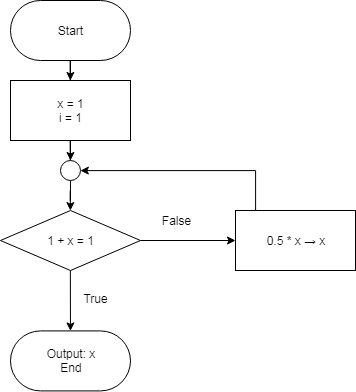
\includegraphics[width=0.4\textwidth]{graphics/machine_epsilon_flowchart}
        \caption{algorithm to find the relative machine precision}\label{fig:epsilon}
      \end{figure}
\begin{proof}
    By definition \(\tau = \frac{1}{2^{-t}}\). Consider \(\text{rd}_t(\frac{1}{2^{t+1}})\). This is by definition rounded to 0, but \(\text{rd}_t(\frac{1}{2^{t}})\) is not. Therefore, let \(x_p\) be the output of the algorithm. Then, \(p = t\) and we have \(x_p = \tau\).
\end{proof}
\end{theorem}

\begin{theorem}
    Using a computer, the relative machine precision can be computed in the following manner
    \begin{equation*}
        \tau = \left|\frac{7}{3} - \frac{3}{4} - 1\right|
    \end{equation*}
\begin{proof}
    We will first evaluate \(\frac{7}{3} - \frac{4}{3}\). We have
    \begin{align}
        \text{rd}_t(\frac{7}{3}) &= \text{rd}_t((10.\overline{01})_2) = \text{rd}_t((0.10\overline{01})_2 \times 2^2) \\
        \text{rd}_t(\frac{4}{3}) &= \text{rd}_t((1.\overline{01})_2) = \text{rd}_t((0.1\overline{01})_2 \times 2^1)
    \end{align}
    The decimal places of the two numbers only differ in placing. Therefore, if we wound the two numbers above one will be rounded up and the other will be rounded down, and we have
    \begin{equation*}
        \left|\text{rd}_t(\frac{7}{3}) - \text{rd}_t(\frac{4}{3})\right| = 2^2 \cdot \sum_{i=1}^{t} \frac{1}{2} - \frac{1}{4} + 0 + \dots + 0 + \frac{1}{2^t} = 1 + \frac{1}{2^t}
    \end{equation*}
    If we subtract \(1\) from the last term, we get \(\tau = \frac{1}{2^t}\) as desired.
\end{proof}
\end{theorem}